\documentclass{beamer}
%\usetheme{Madrid} % My favorite!
%\usetheme{Boadilla} % Pretty neat, soft color.	
\usetheme{default}
%\usetheme{Warsaw}
%\usetheme{Bergen} % This template has nagivation on the left
%\usetheme{Frankfurt} % Similar to the default 
%with an extra region at the top.
%\usecolortheme{seahorse} % Simple and clean template
%\usetheme{Darmstadt} % not so good
% Uncomment the following line if you want %
% page numbers and using Warsaw theme%
% \setbeamertemplate{footline}[page number]
%\setbeamercovered{transparent}
%\setbeamercovered{invisible}
% To remove the navigation symbols from 
% the bottom of slides%
\setbeamertemplate{navigation symbols}{} 
%

%\usepackage{subfig}
\usepackage{amsmath}    % need for subequations
\usepackage{verbatim}   % useful for program listings
\usepackage{color}      % use if color is used in text
\usepackage{subfigure}  % use for side-by-side figures
\usepackage{hyperref}   % use for hypertext links, including those to external documents and URLs
\usepackage{amssymb,latexsym, amsmath}
\usepackage{graphicx}
\usepackage{amsthm}
\usepackage{multirow}
\usepackage{float}
%\usepackage{subcaption}
%\usepackage{caption} 
%\usepackage{subcaption}
%\usepackage{bm} % For typesetting bold math (not \mathbold)
%\logo{\includegraphics[height=0.6cm]{yourlogo.eps}}

\theoremstyle{definition}
\newtheorem{defi}{Definition}
\newtheorem{proposition}{Proposition}%\newtheorem{lemma}{Lemma}
%\graphicspath{{graphs//}}

\title{Ambiguity Insurance and Learning}


\date{\today}
% \today will show current date. 
% Alternatively, you can specify a date.
%
\begin{document}
%
\begin{frame}
\titlepage
\end{frame}
%--------------------------------------------------------------------------------------------e}
%--------------------------------------------------------------------------------------------%

\begin{frame}
\frametitle{Motivation}
Study Optimal Insurance in world where agents face Knightian uncertainty 

\begin{itemize}
	\item With Knightian uncertainty there is feedback between \emph{Risk Perceptions} and \emph{Risk Sharing}.
	\item This link affects how optimal risk sharing schemes look.
\end{itemize}
\end{frame}
%%% Notes

% 1 What do you mean by Knigtian uncertainty - Agents possibly entertaint more than one probablity specification for the randomness in the world. To complete a description of how agents behave in this setting we must specify a theory of how they deal with this multiplicity. Most models of ambiguity try to recast the decision making problem by positing a prioir selection rule confirming certain behavioral regularities.



\begin{frame}
\textbf{Goal :} \emph{Identify the key mechanism affecting insurance in \emph{stylized} environments differing in two dimensions - market completeness and nature of ambiguity}
\vspace{4mm}
\begin{columns}
  \begin{column}{0.5\textwidth}
  \textbf{Market structure}
    \begin{itemize}
\item \small Complete markets 
	\item  \small Exogenously incomplete markets - Bond economy
	\item \small  Endogenously incomplete markets - Private information frictions
   \end{itemize}
  \end{column}
  \begin{column}{0.5\textwidth}
  \textbf{Ambiguity}
     \begin{itemize}
     \item[]
\item \small  Uncertainty about endowment shocks  (observable)
\item \small  Uncertainty about parameters (regimes) (unobservable)
     \end{itemize}
  \end{column}
\end{columns}

\end{frame}
%--------------------------------------------------------------------------------------------%
%%Notes

% I want to study the qualitative mechanics of how these two dimensions - Market structure and Ambiguity interact


\begin{frame}
\frametitle{Basic Mechanism - Simple Example}

Consider a simple example 
\begin{enumerate}
	\item $K$ agents - $u(c)=\frac{c^{1-\gamma}}{1-\gamma}$. 
	\item $Y(z)$ be a risky endowment with support  $[\underline{Y} \quad \bar{Y}]$
\item Agents do not trust the distribution of $Y$ but have a common reference point - $p(y)$ 
\end{enumerate}

Denote a feasible risk sharing arrangement by $\eta = [\eta_1 \dots \eta_K]$ such that $\sum \eta_i=1$

\end{frame}
%--------------------------------------------------------------------------------------------%




\begin{frame}
\frametitle{Basic Mechanism - Simple Example}
\[V^R (\eta_i)=\min_{m}\mathbb{E}m[u(\eta_iY)+\theta\log(m)]\]
such that 
$Em=1$
The choice for $m^*$
\[m_i^*\propto \exp\left\{\frac {-\eta^{1-\gamma}_iy^{1-\gamma}}{\theta(1-\gamma)}\right\}\]

An ex-post Bayesian interpretation : Agents have (diverse) priors given by $p(y)m^*_i(y)$. Note that this depends on $\eta_i$ as long as $\gamma \neq 1$.

\end{frame}


\begin{frame}
\frametitle{Basic Mechanism - Simple Example}
\begin{proposition}
Let $p^*_i=p(y)m^*_i(y)$
\label{propo-1}
\begin{enumerate}
	\item $\lim_{\eta_i \to 0} p_i^*(\underline{Y})=p(\underline{Y}) \quad \gamma < 1$
	\item $\limsup_{\eta_i \to 0} p^*(\underline{Y})=1  \quad \gamma > 1$
\end{enumerate}
\end{proposition}
Agents with low shares of aggregate endowment are ``relatively'' more optimistic when the there is a \textbf{lower bound} on the utility.
\end{frame}




\begin{frame}
\frametitle{Insurance and Heterogeneous Beliefs}
There are 3 broad ways of modeling agents with diverse beliefs
\begin{enumerate}
	\item Exogenous 
	\item Asymmetric Information : Different Information  
	\item Rational Inattention  : Differences in processing of Information
	
\end{enumerate}

\textbf{Model Ambiguity : Agents `choose' to have different beliefs because their continuation values vary differently. }
\end{frame}

%--------------------------------------------------------------------------------------------%


\begin{frame}
\frametitle{Setup}
	\begin{enumerate}
		\item \textbf{Agents}  : $I$ is the  set of agents, where $I= \{1,2\}$
		\item \textbf{Technology} : Exchange economy

		\item \textbf{Endowments}  : Two Shocks - Size and
                  Distribution of aggregate endowment - $z=(y,s)$

\begin{itemize}
\item Model Space : $\mathcal{M}=\{\alpha_m,\beta_m\}_{m\leq M}$ 
\item $\alpha_m,\beta_m$ parametrize the transition density of $z$
\end{itemize}

Given a model we have $P(z^*|z,m)=\mathbb{P}_{Z}[\alpha_m,\beta_m]$. m follows a Markov process 

$\{\mathcal{M},\mathbb{P}_{M},\pi^0_{M}\}$. With this setup we have the following state-space

\[m_{t+1} | m_t \sim \mathbb{P}_{M}\]
\[z_{t+1}|z_t,m_t \sim \mathbb{P}_{Z}(\alpha_{m_t},\beta_{m_t})\]
 	\end{enumerate}
\end{frame}
\begin{frame}
\frametitle{Transition density  - $P_Z$}
\begin{equation}
\label{mat:Pz}
P_Z(z^*|z,m)=P_{Y} (y^*|y,\alpha_m)P_{S|Y} (s^*|y^*,\beta (y^*)) 
\end{equation}

\[P_Y=\bordermatrix{\text{} &y_l&y_h\cr
                y_l&\alpha  & (1-\alpha)\cr
                y_h&   (1-\alpha) &   \alpha}\]
                
\[P_{S|Y}=\bordermatrix{\text{}&s_l&s_h\cr
                y_l& \beta^l & (1-\beta^l)\cr
                y_h&   \beta^h & (1-\beta^h)}\]
                
Note that $\beta$ is a vector of the same dimension as the dimension of the aggregate endowment shock.
\vspace{2mm}

\small{\emph{With this choice I allow for $s$,$y$ to be correlated but $s$ does not \emph{Granger} cause $y$. This choice can be relaxed but will be useful}}

\end{frame}

%-------------------------------------------------------------------------------------------------------------------------------------------------------%

\begin{frame}
\frametitle{Setup - Preferences}
\textbf{Preferences} : Following Hansen and Sargent [2007] the preferences of the agent are described by 2 sets of objects, 
\begin{itemize}
	\item \textbf{Ambiguity}
%	
$\forall i \in I,$
\begin{enumerate}
	\item Approximating Models :   $\left\langle  P^i_M,P_Z^i, \pi^i \right\rangle$
	\item Entropy Penalty - $\theta_j^i$ where $j=2$ captures the doubts about the hidden state ($m$) and $j=1$ about the observable state ($z$)
\end{enumerate}
\item \textbf{Time and Risk} :
\begin{enumerate}
	\item Risk Aversion - $\gamma^i$
	\item Subjective discount factor - $\delta^i$
\end{enumerate}
 \end{itemize}

\textbf{The agents can have potentially different preferences but I will concentrate on the cases where the only differences in the agent is their endowment stream}
%
\end{frame}


\begin{frame}
\frametitle{Recursive Multiplier Preferences}
Given a stochastic process for consumption given by $c(z)$ we have 
\[\mathcal{Q}_c(\pi,z)=\mathbb{T}^2_{\theta_2}\left[u(c(z))+\delta\mathbb{T}^1_{\theta_1,m} \mathcal{Q}_c^*(\pi^*,z^*)\right]\]
where

\[z^*|z \sim P_Z(z^*|z,m)\]
\[\pi^{*}(m^*)\propto \sum_{m}{\pi(m) P_Z(z^*|z,m)P_M(m^*}|m)\]

\end{frame}

\begin{frame}
\frametitle{Planner's Problem}
Let z=(y,s)

$\mathcal{Q}(v,z,\pi)$ be the maximum lifetime discounted value of agent 1 given that $v$ is the promised lifetime discounted valueof agent 2.

\[\mathcal{Q}(v,z,\pi)=\max_{c,v^*(z^*)} \mathbb{T}_{\theta_2}^{2}\left[u^1(c)+\delta \mathbb{T}_{\theta_1,m}^{1} \mathcal{Q}(v^*,z^*,\pi^*)\right]\]
s.t
\[\mathbb{T}_{\theta_2}^2\left[u^2(y-c)+\delta \mathbb{T}_{\theta_1,m}^{1} v^*\right]\geq v\] 
\[\pi^{*}(m^*)\propto \sum_{m}{\pi(m) P_Z(z^*|z,m)P_M(m^*}|m)\]
\end{frame}
%-------------------------------------------------------------------------------------------------------------------------------------------------------%
\begin{frame}
\frametitle{Planner's Problem - FOC}
\small{
\[u^1_c(c)=\lambda u^2_c(y-c)\]	
\[\left(\sum_{m \in M}\tilde{\pi}^1(m)\tilde{P^1}_z(z^* |z,m)\right)\lambda^*=\lambda\left(\sum_{m \in M}\tilde{\pi}^2(m)\tilde{P^2}_z(z^* |z,m)\right) \]
\[\tilde{P}^1 \propto P_Z\exp\left\{\frac{-\mathcal{Q}(v^*,z^*,\pi^*)}{\theta^1}\right\}\]
\[\tilde{P}^2 \propto P_Z\exp\left\{\frac{-v^*}{\theta^1}\right\}\]
\[\tilde{\pi}^1 \propto \pi \exp\left\{-\frac{ u^1(c)+\delta \mathbb{T}^1_{\theta_1,m} \mathcal{Q}(v^*,z^*,\pi^*) }{\theta^2}\right\}\]
\[\tilde{\pi}^1 \propto \pi \exp\left\{-\frac{u^2(y-c)+\delta \mathbb{T}^2_{\theta_1,m} v^*}{\theta^2}\right\}\]
}
\end{frame}

\begin{frame}
\frametitle{Special cases}
\begin{proposition}
\label{propo-2}
With $\gamma=1$ or $y_{l}=y_{h}$, the risk sharing scheme is independent of $\theta_1$ and $\theta_2$
\end{proposition}
With complete markets for wealth heterogeneity to interact with concerns for model uncertainty we need both features
\begin{enumerate}
	\item Presence of aggregate risk 
	\item ``Non-homotheticity'' of preferences
\end{enumerate}
\end{frame}


\begin{frame}
\frametitle{Insurance arrangements - Ambiguity (I)}
Ambiguity (I) :  $\pi(m')=\delta_{m}(m')$ and $\mathbb{P}_M=\mathbb{I}$.

Let $v^{max}(z)$
\[v^{max}(z)=u[y(z)]+\delta \mathbb{T}^1_{\theta_1,m}v^{max}(z^*)\]

\small{Denote $\eta_{\theta_1}$ be the consumption share of Agent 1. }


\begin{proposition}
As $v\to v^{max}$ we have 
\begin{enumerate}
	\item $\frac{\eta_{\theta_1}[y(z^*)=y_l | y_l,v]}{\eta_{\theta_1}(y_l,v)} > 1 \quad \gamma >1$
	\item  $\frac{\eta_{\theta_1}[y(z^*)=y_l | y_l,v]}{\eta_{\theta_1}(y_l,v)} < 1 \quad \gamma < 1$
\end{enumerate}
\end{proposition}

Remarks
\begin{itemize}
	\item \emph{Only aggregate shocks matter}
	\item \emph{Wealthy (poor) agents ``over (under) -insure'' (relative to benchmark [$\theta_1=\infty$]) in bad states ($\gamma <1)$ }
\[\lim_{\theta_1 \to \infty} \frac{\eta_{\theta_1}[z^*]}{\eta_{\theta_1}[z]}=1\]
\end{itemize}
\end{frame}


\begin{frame}
\frametitle{Insurance arrangements - Ambiguity (II)}

Learning activates two novel mechanisms
\begin{enumerate}
\item \textbf{\emph{Compound Lotteries}}  -  The conditional distribution of the payoff relevant shock $z$  has to \emph{averaged} across models which are themselves distributed according to the some prior $\pi(m)$.

\item \textbf{\emph{Distorted Filtering }} - The agent now has access to data on $z$ which is informative about the hidden state $m$.
\end{enumerate}

\emph{Ambiguity (II) - Agents \emph{non-linearly} average across models and distort the outcome of filtering by applying a twist to the (Bayes) posteriors}
\end{frame}

\begin{frame}
\frametitle{Insurance arrangements - Ambiguity (II) }
%
\begin{enumerate}
	\item $\mathcal{M}_{\alpha} = \{m : \alpha_m=\alpha\}$ 
	\item $\pi_\alpha (\alpha)=\sum_{m \in \mathcal{M}_{\alpha}}{ \pi(m)}$
	\item $V^1(z^*)=Q(z^*,\pi^*,v^*)$ and $V^2(z^*)=v^*(z^*|z,v,\pi)$
\end{enumerate}

Define $F_{m}^i$
\[F_{m}^i=\left(\exp\left \{
\mathbb{T}^1_{\theta_1,m}V^i[z^*]
\right\}
\right)^{\left(\frac{\theta_1-\delta\theta_2}{\theta_1\theta_2}\right)}
\]
\begin{equation}
\label{ratio-lambdastar-2}
P(i)=\frac{\sum_{m}\pi(m)P_Z(z^*|z,m)F^i_m
}
{\sum_{m}\pi(m)P_Z(z^*|z,m)F^i_m
}
\end{equation}
\end{frame}

\begin{frame}
\frametitle{Insurance arrangements - Ambiguity (II) }
\begin{proposition}
\label{propo-5}
%
Let $y(z^*)=y(z^{**})$

\noindent CASE 1 : $\theta_1=\infty,\theta_2 < \infty$
if $P(i)$ in equation\ref{ratio-lambdastar-2} is not independent of i,

%
%
\noindent CASE 2 : $\theta_1 <\infty ,\theta_2 < \infty$
if either $P(i)$ in equation \ref{ratio-lambdastar-2} is not independent of i or we have 
\begin{equation}
\label{eq: delta-vstar-qstar}
V^1(z^*)-V^1(z^{**}) \neq V^2(z^*)-V^2(z^{**}) 
\end{equation}
In both cases consumption is sensitive to the distributional shock
\[c(v(z^*),z^*,\pi^*)\neq c(v(z^{**}),z^{**},\pi^{**})\]
\end{proposition}
\end{frame}

\begin{frame}
\frametitle{Insurance arrangements - Ambiguity (II) }
A few sufficient conditions for \ref{ratio-lambdastar-2} to be independent of i, are
%
\begin{enumerate}
\item $\delta \theta_2=\theta_1$
\item $\beta_m(y^*) = \bar{\beta} \quad \forall m : \pi(m) >0$
\item $\alpha_m = \bar{\alpha} \quad \forall m : \pi(m) >0$
\end{enumerate}
The condition \ref{eq: delta-vstar-qstar} will generally be violated for $v$ different from $\bar{v}[z,\pi]$ if $\pi^{*}[\alpha]$ depends on $s^*$
\end{frame}

\begin{frame}
\frametitle{Insurance arrangements - Ambiguity (II)}
\begin{enumerate}
	\item Sufficient conditions for  consumption to be sensitive to the distributional shock - $s$
	\item Asymmetric and non-linear model averaging  - Agents ``disagree'' about $p(s^*|y^*,y)$
	\item Complete markets  facilitates trade on these shocks  - planner's solution implements them
\end{enumerate}
\end{frame}

\begin{frame}
\frametitle{Pricing Kernel}
Shadow prices :
\[q(z^* |z )=\delta \left(\sum_{m \in M}\tilde{\pi}^1(m)\tilde{P^1}_z(z^* |z,m)\right)\frac{ u'(c^*)}{u'(c)}\]

Let $q^{BM}(z^*|z)$ be the asset prices when $\theta_1,\theta_2=\infty$
\[q^{BM}(z^*|z,\pi) = \delta \sum_{m \in M}{\pi(m)P_{z}(z^*|z,m)} \left(\frac{y(z^*)}{y(z)}\right)^{-\gamma}\]

So we have that $\frac{q(z^*|v,z,\pi)}{q^{BM}(z^*|z,\pi)}=\zeta(z^*|v,z,\pi)$
Where 
\[\zeta(z^*|v,z,\pi)=\underbrace{\left(\frac{\sum_{m \in M}\tilde{\pi}^{1}(m)\tilde{P^1}_z(z^* |z,m)}{\sum_{m \in M}{\pi(m)P_{z}(z^*|z,m)}} \right)}_{Distorted Liklihood} \underbrace{\left(\frac{\eta_1(z^*)}{\eta(z)}\right)^{-\gamma}}_{Over (under) insurance} \]
\end{frame}


\begin{frame}
\frametitle{Pricing Kernel - Market Price of Risk}

Define the Conditional market price for risk 
\[MPR(v,z,\pi)=\frac{\sigma[MRS|z]}{\mu[MRS|z]}\] \footnote{Here the $\mu$ and $\sigma$ is with respect to the common reference model}

\[MRS=\zeta(z^*|v,z,\pi)\left(\frac{y(z^*)}{y(z)}\right)^{-\gamma}\]

\vspace{2mm}
\emph{Since $\zeta$ is symmetric and more spread out in the extremes  $\implies$ MPR as a function of $v$ is U shaped}

\end{frame}


\begin{frame}
\frametitle{Market Price of Risk - Cyclicity}
\begin{proposition}
\label{propo-7}
For $\theta_1,\theta_2=\infty$, the conditional market price of risk is countercylical if and only in $\alpha_m < \frac{1}{2}$. With Ambiguity (I), the conditional market price of risk is higher than the benchmark if $\zeta[z^*]$ satisfies the following restrictions

\begin{subequations}
\label{eq:mprgreaterthanbenchmarkcondition}
\begin{equation}
	\frac{\zeta[y(z^*)=y_h|y(z)=y_l]}{\zeta[y(z^*)=y_l|y(z)=y_l]} \leq 1
\end{equation}
\begin{equation}
	\frac{\zeta[y(z^*)=y_l|y(z)=y_h]}{\zeta[y(z^*)=y_h|y(z)=y_h]} \geq 1
\end{equation}
\end{subequations}

For countercylical market price of risk, a sufficient restriction of $\zeta$ is
\tiny
\begin{equation}
\label{eq:countercylicalmprcondition}
\left(\frac{\zeta[y(z^*)=y_h|y(z)=y_l]}{\zeta[y(z^*)=y_l|y(z)=y_l]}\right)\left(\frac{1+g}{1-g}\right)^{-\gamma}+ \left(\frac{\zeta[y(z^*)=y_l|y(z)=y_h]}{\zeta[y(z^*)=y_h|y(z)=y_h]}\right)\left(\frac{1-g}{1+g}\right)^{-\gamma} <2
\end{equation}
\normalsize
\end{proposition}
\end{frame}

\begin{frame}
\frametitle{Survival}
\emph{In this environment there are two belief selection mechanisms which interact with each other. While the market weeds out incorrect beliefs via wealth transfers and the agents themselves are dealing with multiple priors}

Mechanism - 
\begin{itemize}
\item The rich agent transfers wealth to the poor agents in good times
  - Over insurance channel
\item Pessimism  - Good times often more often than the agent
  perceives
\end{itemize}



\end{frame}

\begin{frame}
\frametitle{Survival-Digression}
Consider a case when the agents differ in the approximating model	,in particular
\begin{enumerate}
\item $P_Z(z^*|z)=P_Z(z^*)=P^2_Z(z^*)$
\item $P_Z^1(z^*) \neq P_Z(z^*)$
\end{enumerate}
%
The FOC of the Planner are 
%
\[\frac{\lambda_{T+1}}{\lambda_{T}} =\left[\frac{\tilde{P}^2_Z(z_{T+1})}{\tilde{P}^1_{Z}(z_{T+1})}\right]\]
%Where 
\[\tilde{P}^1_Z \propto P^1_Z \exp \left\{-\frac{Q_{T+1}}{\theta_1}\right\}\]
\[\tilde{P}^2_Z \propto P_Z \exp \left\{-\frac{V_{T+1}}{\theta_1}\right\}\]
%
\end{frame}



\begin{frame}
\frametitle{Survival-Digression}

Taking logs and iterating backwards we have

\begin{eqnarray*}
\frac{1}{T}\lambda_{T}&=\frac{1}{T}\sum_{t=0}^{T}\log\tilde{m}^2_{t,t+1}-\frac{1}{T}\sum_{t=0}^{T}\log \tilde{m}^1_{t,t+1}+\\ &+ \left( \frac{1}{T}\sum_{t=0}^{T}\log[P_Z(z_{t+1})]\right)\\
&- \left( \frac{1}{T}\sum_{t=0}^{T}\log[P^1_Z(z_{t+1})]\right)]
\end{eqnarray*}


Now if $\lambda_{T}\to \infty$ then we have
\begin{itemize}
\item $V_{T}\to V_{Max}$
\item $Q_{T}\to 0$
\item $\tilde{m}^1_{T,T+1} \to 1$
\item $\tilde{m}^2_{T,T+1} \to \frac{\exp \{-\frac{V_{Max}}{\theta_1}\}}{\mathbb{E}_2 \exp\{-\frac{V_{Max}}{\theta_1}\}} \quad (`m`)$
\end{itemize}
\end{frame}


\begin{frame}
\frametitle{Survival-Digression}
Using the LLN, for large T,

\[\lambda_T=e^{[\mathbb{I}_1 + \mathbb{E} log m]T} \]

Since $\mathbb{E}m=1$, generally $\mathbb{E} log m$ will be negative
and it means that the relative entropy of Agent 1 ($\mathbb{I}_1$) has to sufficiently
high for him to vanish or $\lambda_T$ to diverge.


\end{frame}


\begin{frame}
\frametitle{Planner's Problem - Numerical Example}
I numerically (cubic splines) solve the planners problem for the following calibrations
\begin{enumerate}
	\item $\alpha =[ .5;.9]$
	\item $\beta=[.5 \quad .5 ;.9 \quad .5]$
	\item $\gamma=.5$
	\item $y(z)=\bar{y}(1+g(z))$
	\item $\theta_1=.5$
\item $\theta_2=.5$
	\item $g(z)=-30\%$ if $z=1,2$ and $30\%$ otherwise
\end{enumerate}

\end{frame}

\begin{frame}[label=ResultsComMarket]
\frametitle{Results}
\begin{enumerate}
	\item Consumption Shares \hyperlink{ConsSharesAmb1}{\beamergotobutton{}}
	\item Relative Entropy  \hyperlink{RelEntropy}{\beamergotobutton{}}
	\item MPR - Ambiguity (I) \hyperlink{MPRNoLearning}{\beamergotobutton{}}
	\item MPR - Ambiguity (II) \hyperlink{MPRLearning}{\beamergotobutton{}}
	\item Pareto Shares  \hyperlink{LambdaNoLearning}{\beamergotobutton{}}
\end{enumerate}
\end{frame}


\begin{frame}
\frametitle{Long run dynamics}
In the next few slides I will show results for the following cases
\begin{enumerate}	
\item Ambiguity (I) : $P_M=\mathbb{I}$ and $\pi \in\{0,1\}$ 
\item Ambiguity (II) - Transitory Learning : Same as above but $\pi \in(0 \quad 1)$
\item Ambiguity (II) - Persistent Learning : In this case $P_M$ is such that each model
  can switch with prob $0.1$
\end{enumerate}
\end{frame}




\begin{frame}
\frametitle{Ambiguity (I) - $v_{SS}$}
\begin{figure}[htbp]
\centering
	  \includegraphics[scale=0.4]{Matlab/InfiniteHorizon/Learning/Plots/theta_1_finite/Transitory/VSS.png}

	\caption{\small {This figure plots the ergodic distribution of $v^*$ for $\theta_1,\theta_2 =.5$ and $P_M=\mathbb{I}$}}
	
	\label{fig:VSS_theta_1_finite_transitory}
\end{figure} 
\end{frame}
%
%
%
\begin{frame}
\frametitle{Ambiguity (I) - MPR }
\begin{figure}[htbp]
\centering
	  \includegraphics[scale=0.4]{Matlab/InfiniteHorizon/Learning/Plots/theta_1_finite/Transitory/MPRDraw.png}

	\caption{\small {This figure plots a sample path of MPR from the ergodic distribution for $\theta_1,\theta_2 =.5$ and $P_M=\mathbb{I}$}. The shaded bars have $y(z)=y_l$}

	\label{fig:MPRDraw_theta_1_finite_transitory}
\end{figure} 
\end{frame}

%
%
\begin{frame}
\frametitle{Ambiguity (II) Transitory - $\lambda_{SS}$ - ``Catching up''}
Let $\theta_1=\infty,\theta_2 =0.5$
\begin{figure}[htbp]
\centering
	  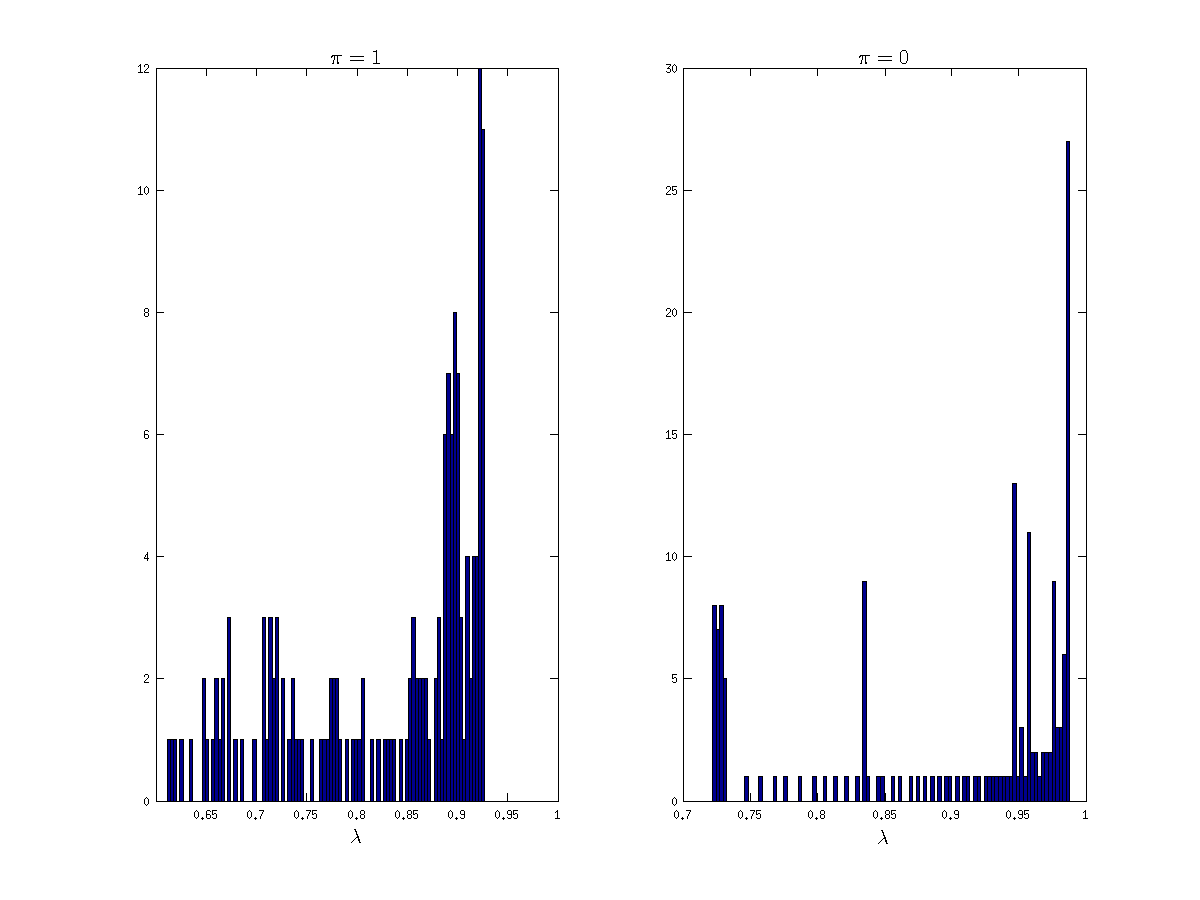
\includegraphics[scale=0.4]{Matlab/InfiniteHorizon/Learning/Plots/theta_1_infty/Transitory/LambdaSS.png}

	\caption{\small {This figure plots the ergodic distribution for $\lambda$ with $\theta_1=\infty,\theta_2 =.5$ and $P_M=\mathbb{I}$}}
	
	\label{fig:LambdaSS_theta_1_infty_transitory}
\end{figure} 
\end{frame}
%
\begin{frame}
\frametitle{Ambiguity (II) Persistent - $v_{SS}$}
\begin{figure}[htbp]
\centering
	  \includegraphics[scale=0.4]{Matlab/InfiniteHorizon/Learning/Plots/theta_1_finite/Persistent/VSS.png}
%
	\caption{\small {This figure plots the ergodic distribution of $v^*$ for $\theta_1,\theta_2 =.5$ and $P_M \neq \mathbb{I}$}}
%	
	\label{fig:VSS_theta_1_finite_persistent}
	\end{figure}
\end{frame}

%
\begin{frame}
\frametitle{Ambiguity (II) Persistent - MPR}
\begin{figure}[htbp]
\centering
	  \includegraphics[scale=0.4]{Matlab/InfiniteHorizon/Learning/Plots/theta_1_finite/Persistent/MPRDraw.png}
%
	\caption{\small {This figure plots a sample path of MPR for $\theta_1,\theta_2 =.5$ and $P_M \neq \mathbb{I}$}. The red bars are periods with $y(z)=y_l$}
	
	\label{fig:MPR_theta_1_finite_persistent}
	\end{figure}
\end{frame}

\begin{frame}
\frametitle{Ambiguity (II) Persistent - $v_{SS}$}
\begin{figure}[htbp]
\centering
	  \includegraphics[scale=0.4]{Matlab/InfiniteHorizon/Learning/Plots/theta_1_infty/Persistent/VSS.png}
%
	\caption{\small {This figure plots the ergodic distribution of $v^*$ for $\theta_1=\infty,\theta_2 =.5$ and $P_M \neq \mathbb{I}$}}
	
	\label{fig:VSS_theta_1_infty_persistent}
\end{figure}
\end{frame}
%
%
\begin{frame}
\frametitle{Ambiguity (II) Persistent - MPR}
\begin{figure}[htbp]
\centering
	  \includegraphics[scale=0.4]{Matlab/InfiniteHorizon/Learning/Plots/theta_1_infty/Persistent/MPRDraw.png}

	\caption{\small {This figure plots a sample path of MPR for $\theta_1=\infty,\theta_2 =.5$ and $P_M \neq \mathbb{I}$. The red bars are $y(z)=y_l$}}
%	
	\label{fig:MPR_theta_1_infty_persistent}
	\end{figure}
\end{frame}
%%------------------------------------------------------------------------------------------------------------------------------
\begin{frame}
\frametitle{Review Complete Markets}
\begin{enumerate}
	\item Wealth $\implies$ `ex-post' beliefs $\implies$ Insurance demands $\implies$ Wealth 
	\item Hidden states $\implies$ consumption sensitive to distributional shocks
	\item Lower bounds on utility matter 
\end{enumerate}
In the next two parts market completeness is relaxed. 
\begin{enumerate}
	\item Bond economy - \emph{self insurance} channel : Relative optimism increases in wealth
	\item Private information - Insurance and incentives interact
\end{enumerate}
\end{frame}



\begin{frame}
\frametitle{Incomplete Markets - Simple Example}
Consider an agent with a (truncated ) Gaussian risky endowment $Y$. He has risk
free assets which pay $b$. 
\[c(y,b)=y+b\]

\[V^R (b)=\min_{m}\mathbb{E}m[u(c)+\theta\log(m)]\]
such that 
$Em=1$
 The choice for $m^*$
\[m_i^*(y,b)\propto \exp\left\{\frac {-(y+b)^{1-\gamma}}{\theta(1-\gamma)}\right\}\]

\end{frame}


\begin{frame}
\frametitle{Incomplete Markets - Simple Example}

Remarks

\begin{itemize}
\item  An ex-post Bayesian interpretation : Agents have (diverse) priors
given by $p(y)m^*_i(y,b)$ depending on wealth
\end{itemize}
\begin{proposition}
For every $b$  there exists a threshold $\bar{y}(b)$ such that $\frac{\partial m(y,b)}{\partial b} >0 \quad \text{iff} \quad  y>\bar{y}(b)$
\end{proposition}

 \emph{The intuition is that with higher $b$ the relative fluctuations in $y$ are not large enough to distort the distribution of $y$. Large assets provide the buffer for self-insurance and hence eliminate or reduce concerns for model uncertainty.}
\end{frame}



\begin{frame}
\frametitle{Incomplete Markets - Simple Example}
\begin{figure}[htbp]
\centering
	  \includegraphics[scale=0.4]{Matlab/IncompleteMarkets/Plots/StaticBondEconomy.png}

	\caption{\small{This figure shows the reference and worst case models for two levels of assets in the static example with $\theta=1$,$\gamma=0.5$}}
	\label{fig:StaticBondEconomy}
\end{figure} 

\end{frame}

\begin{frame}
\frametitle{Incomplete Markets - Simple Example}
\begin{figure}[htbp]
\centering
	  \includegraphics[scale=0.4]{Matlab/IncompleteMarkets/Plots/StaticYBar.png}

	\caption{\small{This figure plots $\bar{y} (b)$ for the static example with $\theta=1$,$\gamma=0.5$. The shaded region are realizations of $y$ for which $m^*_b(y,b)>0$}}
	\label{fig:StaticYBar}
\end{figure} 
\end{frame}


\begin{frame}
\frametitle{Incomplete Markets - General Case}
\begin{enumerate}
	\item Risk free bonds in zero net supply
	\item No aggregate risk i.e $y_{l}=y_{h}$
	\item Distributional shock  : $s^*|s \sim P_S[m]$ 
	\[P_S(s^*|s,m)=\bordermatrix{~ & s_l & s_h \cr
														s_l & \alpha^S(m) & 1-\alpha^S(m) \cr
														s_h & 1-\alpha^S(m) & \alpha^S(m) \cr} \]
	\item Parameter regimes  : $m$
	\[m^* | m  \sim \mathbb{P}_{M}\]													
	\end{enumerate}
\emph{With the zero aggregate supply of bonds and common initial priors - $\pi_0$, the sufficient state variables for this economy are $(B^1, s, \pi)$ }

\end{frame}

\begin{frame}
\frametitle{HH problem- Agent 1 }
\noindent Given bond prices $q$, let $Q^i(b,B^1,s,\pi)$ be the value of Agent i with assets b and aggregate state $(B^1,s,\pi)$

\begin{equation}
\label{BEAgent1ValueFunction}
\mathcal{Q}^1(b,B^1,s,\pi)=\max_{c,b^*} { \mathbb{T}^2_{\theta_2} \left[u(c)+\delta \mathbb{T}^1_{\theta_1,m}\mathcal{Q}^1 (b^*,B^{1*},s^*,\pi^*)\right]}
\end{equation}
subject to
\begin{subequations}
\begin{equation}
c+qb^*=ys+b
\end{equation}
\begin{equation}
\pi^* \propto \sum_{m}{P_M(m^*|m)P_S(s^*|s,m)\pi(m)}
\end{equation}
\begin{equation}
b^* \geq \underbar{b}^1(s)
\end{equation}
\end{subequations}

Where $\underbar{b}^1(s)$ is the natural debt limit for Agent 1 in state $s$
\end{frame}





\begin{frame}
\frametitle{HH problem- Agent 2 }
\begin{equation}
\label{BEAgent2ValueFunction}
\mathcal{Q}^2(b,B^1,s,\pi)=\max_{c,b^*} { \mathbb{T}^2_{\theta_2} \left[u(c)+\delta \mathbb{T}^1_{\theta_1,m}\mathcal{Q}^2 (b,B^{1*},s^*,\pi^*)\right]}
\end{equation}
subject to
\begin{subequations}
\begin{equation}
c+qb^*=y(1-s)+b
\end{equation}
\begin{equation}
\pi^* \propto \sum_{m}{P_M(m^*|m)P_S(s^*|s,m)\pi(m)}
\end{equation}
\begin{equation}
b^* \geq \underbar{b}_2 (s)
\end{equation}
\end{subequations}
Where $\underbar{b}^2(s)$ is the natural debt limit for Agent 2 in state $s$. 
\end{frame}




\begin{frame}
\frametitle{Equilibrium}
Given $(B^{1}_{-1,0}, s_0, \pi_0)$ a recursive comptetitive equilibrium is set of value function,policy rules for each agent - $\{\mathcal{Q}^i,\mathcal{B}^i\}_{i=1,2}$ and bond prices $q$ such that given $q$, the value functions and policy rules solve the agents problems and bonds markets clear
\[q(B^1,s,\pi) : \mathcal{B}^1(B^1,B^1,s,\pi,q)+  \mathcal{B}^2(-B^1,B^1,s,\pi,q)=0\]
\end{frame}




\begin{frame}
\frametitle{A Minimally Stochastic Case}
\begin{enumerate}
	\item $s_1|s_0 \sim P_S[s^*|s,m]$
	\item $s_{t+1}=s_{t}$ for $t\geq1$ 
\end{enumerate}

\begin{proposition}
\label{propo-10}
There exists a $\underbar{B}^1_{-1,0}[s,\pi]$ such that $\lim_{b\to \underbar{B}^1_{-1,0}} \mathcal{B}^{1,0}(b,\underbar{B}^1_{-1,0},s,\pi,q) = -\frac{ys_l}{1-\delta}$. Further we also have 
\[\lim_{b \to \underbar{B}^1_{-1,0}}\bar{y}[\mathcal{B}(b,\underbar{B}^1_{-1,0},s,\pi,q)] = ys_l\]
\end{proposition}
\end{frame}



\begin{frame}
\frametitle{Parameter Values}
\[\begin{tiny}\begin{tabular}{|l|c|}
\hline
&\textbf{Description}\\\hline
\textbf{Agggregate Income ($y$)}&10.00\\\hline
\textbf{Low share of Endowment ($s_l$)}&0.30\\\hline
\textbf{High share of Endowment ($s_h$)}&0.70\\\hline
\textbf{Probability of switching - Model 1 (1-$\beta_1$)}&0.50\\\hline
\textbf{Probability of switching - Model 2 (1-$\beta_2$)}&0.10\\\hline
\textbf{Risk Aversion ($\gamma$)}&1.00\\\hline
\textbf{Subjective Discount Factor($\delta$)}&0.80\\\hline
\textbf{Ambiguity - Observable State ($\theta_1$)}&2.00\\\hline
\textbf{Ambiguity - Hidden State ($\theta_2$)}&0.50\\\hline
\end{tabular}
\end{tiny}\]
\end{frame}
\begin{frame}
\frametitle{Bond Prices}
\begin{figure}[htbp]
\centering
	  \includegraphics[scale=0.4]{Matlab/IncompleteMarkets/InfiniteHorizon/Plots/theta_1_finite/Transitory/figEBondPricesNoLearning.png}

	\caption{\small{The figure plots averaged bond prices as a function of Agent-1's level of assets.} }
 
	\label{fig:figEBondPricesNoLearning}
\end{figure} 
\end{frame}


\begin{frame}
\frametitle{Distorted Transitions}
\begin{figure}[htbp]
\centering
	  \includegraphics[scale=0.4]{Matlab/IncompleteMarkets/InfiniteHorizon/Plots/theta_1_finite/Transitory/figDistP.png}

	\caption{ The plots above depict $\tilde{P}^1(s^*|s,m)$. The left (right) column is the IID (NonIID) model and the dotted(solid) line refers to $s^*=s_l$ ($s_h$). The top (bottom) panels refer to $s=s_l (s_h)$}
 
	\label{fig:DistP}
\end{figure} 
\end{frame}



\begin{frame}
\frametitle{Distorted Priors}
\begin{figure}[htbp]
\centering
	  \includegraphics[scale=0.4]{Matlab/IncompleteMarkets/InfiniteHorizon/Plots/theta_1_finite/Transitory/figDistPi.png}

	\caption{ \small{This plots $\tilde{\pi}^1$ given $\pi=\frac{1}{2}$. The top (bottom) panel is $s=s_l$ ($s_h$) }}
 
	\label{fig:figDistPi}
\end{figure} 
\end{frame}


\begin{frame}
\frametitle{Erogdic Wealth Distribution}
\begin{figure}[htbp]
\includegraphics[width=0.5\textwidth]{Matlab/IncompleteMarkets/InfiniteHorizon/Plots/theta_1_finite/Transitory/figBstarSim.png}
	  \hfill \includegraphics[width=0.5\textwidth]{Matlab/IncompleteMarkets/InfiniteHorizon/Plots/theta_1_finite/Persistent/figBstarSim.png}

\caption{\small {The figure plots the ergodic wealth distribution of $B^1$. The left panel is the transient learning case with IID model and the right panel refers to $P_M\neq\mathbb{I}$}}
\end{figure} 
\end{frame}

\begin{frame}
\frametitle{Heterogenous Priors}
\begin{figure}[htbp]
\centering
	  \includegraphics[scale=0.4]{Matlab/IncompleteMarkets/InfiniteHorizon/Plots/theta_1_finite/Persistent/figPiDiffSim.png}

	\caption{\small{This plots the ergodic distribution of $\tilde{\pi}_{gap}=\frac{|\tilde{\pi}^1-\tilde{\pi}^2|}{\tilde{\pi}}$ }}
 
	\label{fig:figPiDiff}
\end{figure} 
\end{frame}

\begin{frame}
\frametitle{Endogenously incomplete markets}
I study a 2 period version of the  economy with the private
information as a way of formalizing endogenous incompleteness.
\begin{enumerate}
\item No aggregate risk
\item Private information about income in period 2
\item \emph{Continuation values have to satisfy incentive compatibility}

\end{enumerate}
\end{frame}


\begin{frame}
\frametitle{Private Information Setup }
I modify the earlier setup with complete markets in the spirit of  Green and Oh (1991)

Compress the state space to $z_1$, $z_2$ such that

\begin{table}[h]
  \centering
  \begin{tabular}[h]{l c c}
    
& Agent 1 & Agent 2 \\
$z_1$ & $ys_l$ & $y s_h$  \\
$z_2$ & $ys_h$ & $ys_l$ \\
 
  \end{tabular}
  \caption{Endowments}
  
\end{table}

Let $\{P_Z(m)\}_m  $ be the transition matrices for IID model 1 (m=1) and
Non- IID model 2 (m=2)


\end{frame}



\begin{frame}
\frametitle{Incentives}
Let $\Delta=y(s_h-s_l)$ 
\begin{table}[h]
  \centering
  \begin{tabular}[h]{l c c}
    
& Agent 1 & Agent 2 \\
$z^*_1$ & $c(z^*_1)\geq c(z^*_2)-\Delta$ & $y-c(z^*_1)\geq y-c(z^*_2)+\Delta$  \\
$z^*_2$ & $c(z^*_2)\geq c(z^*_1)+\Delta$ & $y-c(z^*_2)\geq y-c(z^*_1)-\Delta$  \\
 
  \end{tabular}
  \caption{Incentive Constraints}
  
\end{table}


From the above table we obtain,
\[c(z^*_2)=c(z^*_1)+\Delta\]
or 
\[v^*(z^*_1) = u[u^{-1} \left[v^*(z^*_2)\right] +
  y(s_h-s_l)] \]


\end{frame}


\begin{frame}
\frametitle{Effecient allocations - Planner's Problem}


$\mathcal{Q}(v,z,\pi)$ be the maximum lifetime discounted utility of agent 1 given that $v$ is the promised lifetime discounted utility of agent 2.

\[\mathcal{Q}(v,z,\pi)=\max_{c,v^*(z^*_1),v^*(z^*_2)  } \mathbb{T}_{\theta_2}^{2}\left[u^1(c)+\delta \mathbb{T}_{\theta_1,m}^{1} \mathcal{Q}(v^*,z^*,\pi^*)\right]\]
s.t
\[\mathbb{T}_{\theta_2}^2\left[u^2(y-c)+\delta
  \mathbb{T}_{\theta_1,m}^{1} v^*\right]\geq v \quad (\text{`PK'})\] 

\[v^*(z^*_1) = \underbrace{u[u^{-1} \left[v^*(z^*_2)\right] +
  y(s_h-s_l)]}_{\text{Value of misreporting in $z^*_1$ }}  \quad (\text{`IC'})\]

\[\pi^{*}(m^*)\propto \sum_{m}{\pi(m) P_Z(z^*|z,m)P_M(m^*}|m)\]
\end{frame}



\begin{frame}
\frametitle{Private Information - FOC}
Let $\lambda$ and $\mu$ be the Lagrange multipliers on PK and IC
\[u_c[c]-\lambda u_c[y-c]=0\]
\[\left[\sum_{m}{\tilde{\pi}^1(m)\tilde{P}^1_z(z^*_1 | z,m)}\right]
Q^*_v [z^*_1] +\left[\sum_{m}{\tilde{\pi}^2(m)\tilde{P}^2_z(z^*_1 |
    z,m)}\right]  \lambda  + \mu =0\]
\begin{align*}
\left[\sum_{m}{\tilde{\pi}^1(m)\tilde{P}^1_z(z^*_2 | z,m)}\right]
Q^*_v [z^*_2] &+ \left[\sum_{m}{\tilde{\pi}^2(m)\tilde{P}^2_z(z^*_2 |
    z,m)}\right]  \lambda\\
& -\mu\left( \frac{u_c[u^{-1} \left[v^*(z^*_2)\right]+ 
    y(s_h-s_l)]}{u_c[u^{-1} \left[v^*(z^*_2)\right]]}\right)=0
\end{align*}

\emph{$\tilde{\pi}^i $ and $\tilde {P}^i_z$ are the respective
  distorted probabilities of the hidden state and the observable state}
\end{frame}

%%%%%%%%% Note on Optimal Contract %%%%%%%%%%%%%%%
\begin{frame}
\frametitle{Optimal Insurance}
Let 

\begin{itemize}
	\item $\mathcal{C}^0$ be the consumption of Agent 1 in $t=0$
\item  $\mathcal{C}^1$ be $t=1$ the consumption if $z(t_1)$ is reported to be $z_1$
\item $\beta(z)=\sum_{m}{\pi(m)P_Z(z_1|z,m)}$ 

\end{itemize}
Define $C^1_{\infty} = \lim_{\theta_1,\theta_2 \to \infty} \mathcal{C}^1$ 

\begin{proposition}
The optimal incentive compatible consumption plan is given by the following allocation - $\langle \mathcal{C}^0(z)[\lambda(v,z)],\{\mathcal{C}^{1}[\lambda(v,z)],\mathcal{C}^{1}[\lambda(v,z)]+\Delta\}\rangle$. This contract has the following features.

There exists a $\bar{\lambda}(z)$ such that 
\begin{itemize}
	\item $\mathcal{C}^{1}[\lambda] > \mathcal{C}^{1}_{\infty}[\lambda] \quad \lambda < \bar{\lambda}(z)$
	\item $\mathcal{C}^{1}[\lambda] < \mathcal{C}^{1}_{\infty}[\lambda] \quad \lambda > \bar{\lambda}(z)$
\end{itemize}

Further $\bar{\lambda}(z)=1$ if $\beta(z)=\frac{1}{2}$
\end{proposition}

\end{frame}

\begin{frame}
\frametitle{Insurance contract}
\begin{figure}[htbp]
\centering
	  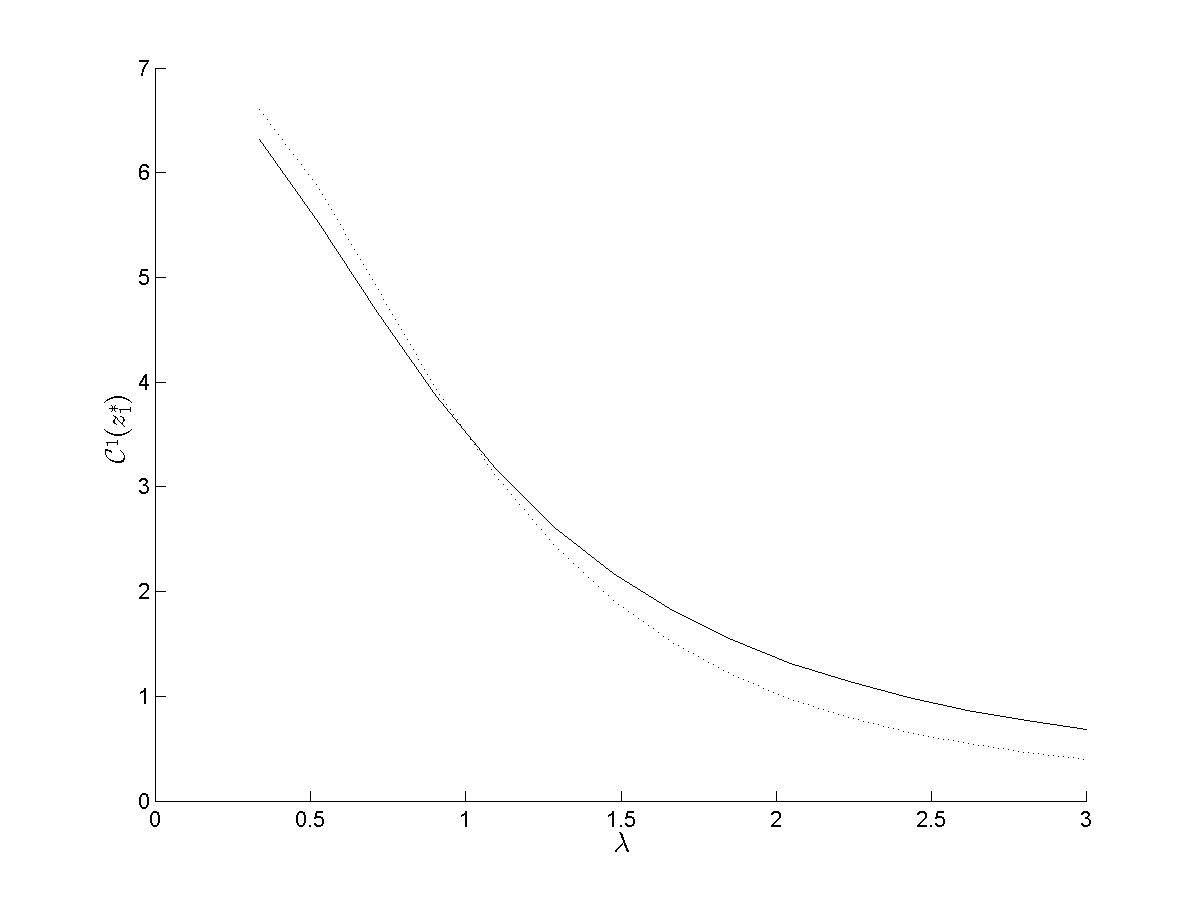
\includegraphics[scale=0.5]{Matlab/PrivateInformation/Plots/StaticPIConsumptionPlan.png}

	\caption{The plot depicts consumption of Agent 1 in $t=1$, state $z_1$. The dotted line is the benchmark without concerns for model ambiguity.}
	\label{fig:BondEconomyOucomes}
\end{figure} 

\end{frame}
\begin{frame}
\frametitle{Insurance and Incentives} 
\emph{How do insurance and incentives interact}
\begin{enumerate}
	\item The IC constraint $\implies $  $c(z^*_2)-c(z^*_1)=\Delta$. This holds independently of attitudes towards ambiguity
	
	\item As compared to case without ambiguity, there are two forces which distort the optimal insurance scheme. Consider the situation when the current sate ($z(t_0)=z_1$). 
	
\begin{itemize}
	\item $\mathcal{C}^1$ dimishes with $\lambda$
	
	\[\lambda \to \infty \implies \frac{c^*(z^*_1)}{y-c^*(z^*_1)} \to 0\]
	
	However the IC constraint restricts the consumption plan to be $[c^(z^*_1),c^(z^*_1)+\Delta]$. 
	\end{itemize}
\end{enumerate}
	\end{frame}
	
	
	
	\begin{frame}
	\frametitle{Insurance and Incentives} 
	\begin{itemize}
	\item Since utility is concave, $u(c+\Delta)-u(c)$ is decreasing in  $c$  for a fixed $\Delta$. 
		\[\tilde{\beta}^1 > \beta > \tilde{\beta}^2\]
	
	
	\item Optimal insurance requires the planner to allocate higher consumption to agents who perceive the given state more likely. However this channel only appears with endogenous beliefs when agents fear model misspecification. So given everything else as $\lambda \to \infty $ Agent 1's consumption $c^*(z^*_1)$ is higher than what he would get without ambiguity. Since the agents are otherwise symmetric, the converse is true when $\lambda \to 0$. 
\end{itemize}

\end{frame}


\begin{frame}
\frametitle{Dynamic Incentives and Ambiguity}
Now we setup the Planner's problem with dynamic private information.

\emph{This modifies the above setup even with two periods. Unlike before the current state is also unobserved by the Planner}

\begin{enumerate}
	\item This introduces a new lever for the Planner to provide incentives in presence of model uncertainty - \emph{Continuation Plans}
	\item The Planner faces a choice of how to provide incentives 
	
\begin{itemize}
	\item Distorting  the current consumption menu
	\item Distort continuation plans
\end{itemize}

\end{enumerate}
\end{frame}


\begin{frame}
\frametitle{Dynamic Incentives and Ambiguity}
It is useful to define the ex-ante version of $Q$ - The optimum value to Agent 1 ($Q^0$)
\footnote{$z\_$ is the reported state in the previous period}

\[Q^0(v^0,z \_)=\max_{c(z),\bar{v}^*(z)}{\mathbb{T}^1_{\theta,z\_}\left\{ u[c(z)]+\delta Q^{0}[\bar{v}^{*}(z),z]\right\}}\] 
s.t
\[\mathbb{T}^1_{\theta,z\_}\left\{ u[y-c(z)]+\delta \bar{v}^{*}(z)\right\}\geq v^0 \quad (\text{`PK'})\]

\end{frame}

\begin{frame}
\frametitle{Dynamic Incentive Constraints}
Let $\Delta=y(s_h-s_l)$ 
\small{
\begin{table}[h]
  \centering
  \begin{tabular}[h]{l |p{5cm} | p{4cm}}    
& Agent 1 & Agent 2 \\
\hline
$z_1$ & $u[c(z_1)]+\delta Q^{0}[\bar{v}^{*}(z_1),z_1]\geq u[c(z_2)-\Delta]+\delta Q^{0}[\bar{v}^{*}(z_2),z_1]$ & $u[y-c(z_1)]+\delta \bar{v}^{*}(z_1)\geq u[y-c(z_2)+\Delta]+\delta \bar{v}^{*}(z_2)$  \\
 & &\\
$z_2$ & $u[c(z_2)]+\delta Q^{0}[\bar{v}^{*}(z_2),z_2]\geq u[c(z_1)+\Delta]+\delta Q^{0}[\bar{v}^{*}(z_1),z_2]$ & $u[y-c(z_2)]+\delta \bar{v}^{*}(z_2)\geq u[y-c(z_1)-\Delta]+\delta \bar{v}^{*}(z_1)$  \\
  \end{tabular}
  \caption{Dynamic Incentive Constraints}
\end{table}
}
Let $\mu^i_z$ denote the multiplier on incentive constraint for agent i in state z
\end{frame}


\begin{frame}
\frametitle{Optimal Benchmark Contract - Characterization}
Numerical investigation reveals a few features of the Optimal Contract for the IID case

\begin{proposition}
$ \exists \bar{\lambda} \quad \&\quad \epsilon > 0$ such that
\begin{enumerate}
	\item $\mu^1_{z_2} > 0 \quad  \forall \lambda \leq \bar{\lambda} +\epsilon$
	\item $\mu^2_{z_1} > 0 \quad  \forall \lambda \geq \bar{\lambda} -\epsilon$
\end{enumerate}
\end{proposition}

Further the $\epsilon$ is independent of $\theta$
\end{frame}


\begin{frame}
\frametitle{Multipliers and binding constraints}
\begin{figure}[htbp]
\centering
	  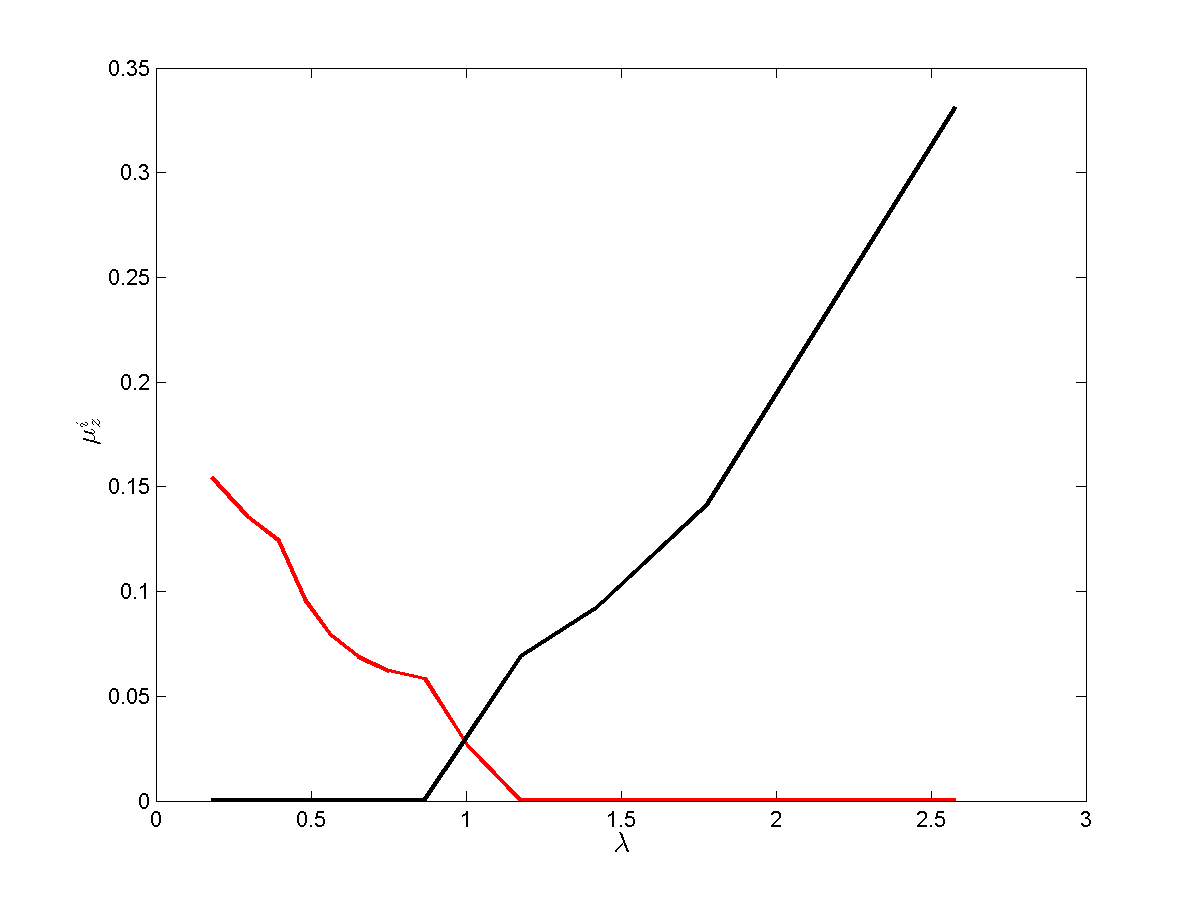
\includegraphics[scale=0.4]{Matlab/PrivateInformation/Plots/BindingMultipliers.png}
	\caption{ This figure plots the multiplier on the binding incentive
 constraint. The red line refers to $\mu^1_2$ - Agent 1 State $z_2$ and the
 black line refers to $\mu^2_1$ - Agent 2 state $z_1$. The dotted line is
 $\theta=\infty$ case}
	\label{fig:BindingMultipliers}
\end{figure} 
\end{frame}


\begin{frame}
\frametitle{Optimal time 0 - Consumption Menu- Irrelevance of $\theta$}
\emph{Since the binding mechanics of $\mu$ are independent of $\theta$, we have that the initial period consumption plan as a function of $\lambda$ has the same property }
\begin{figure}[htbp]
\centering
	  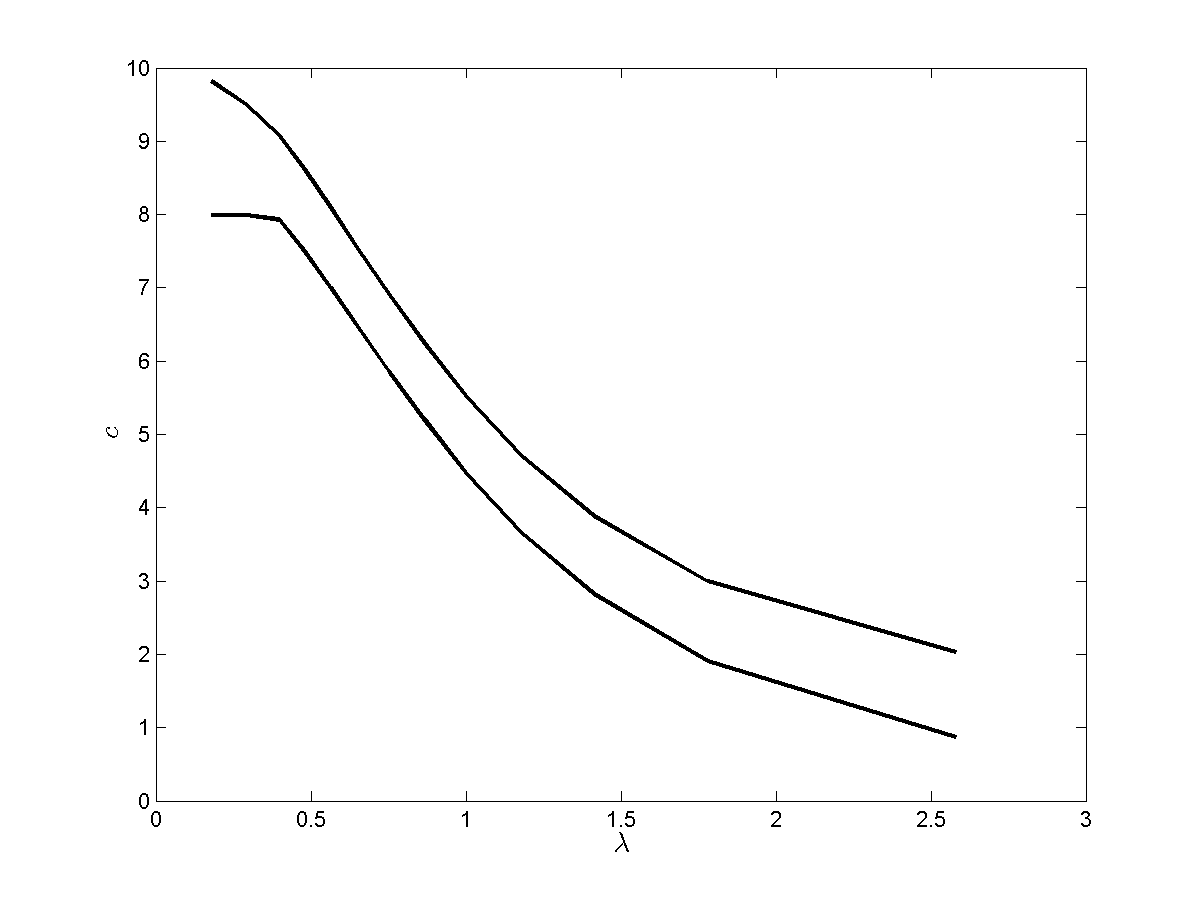
\includegraphics[scale=0.35]{Matlab/PrivateInformation/Plots/CompOptContractCons.png}

	\caption{\small{This plot shows the time-0 consumption plan as a function of $\lambda$. The dotted line represents $\theta=\infty$}}
	\label{fig:CompOptContractCons}
\end{figure} 
\end{frame}

\begin{frame}
\frametitle{Next steps}
\begin{enumerate}
\item Document results for the $\gamma > 1$  
\item Solve the example with dynamic incentives provision
\item Study the infinite horizon versions of incomplete markets - Long run wealth dynamics	
\item Connect to applications and existing literature
\end{enumerate}
\end{frame}

\begin{frame}[label=ConsSharesAmb1]
\frametitle{Consumption Shares - Ambiguity (I)}
\begin{figure}[htbp]
\centering
	  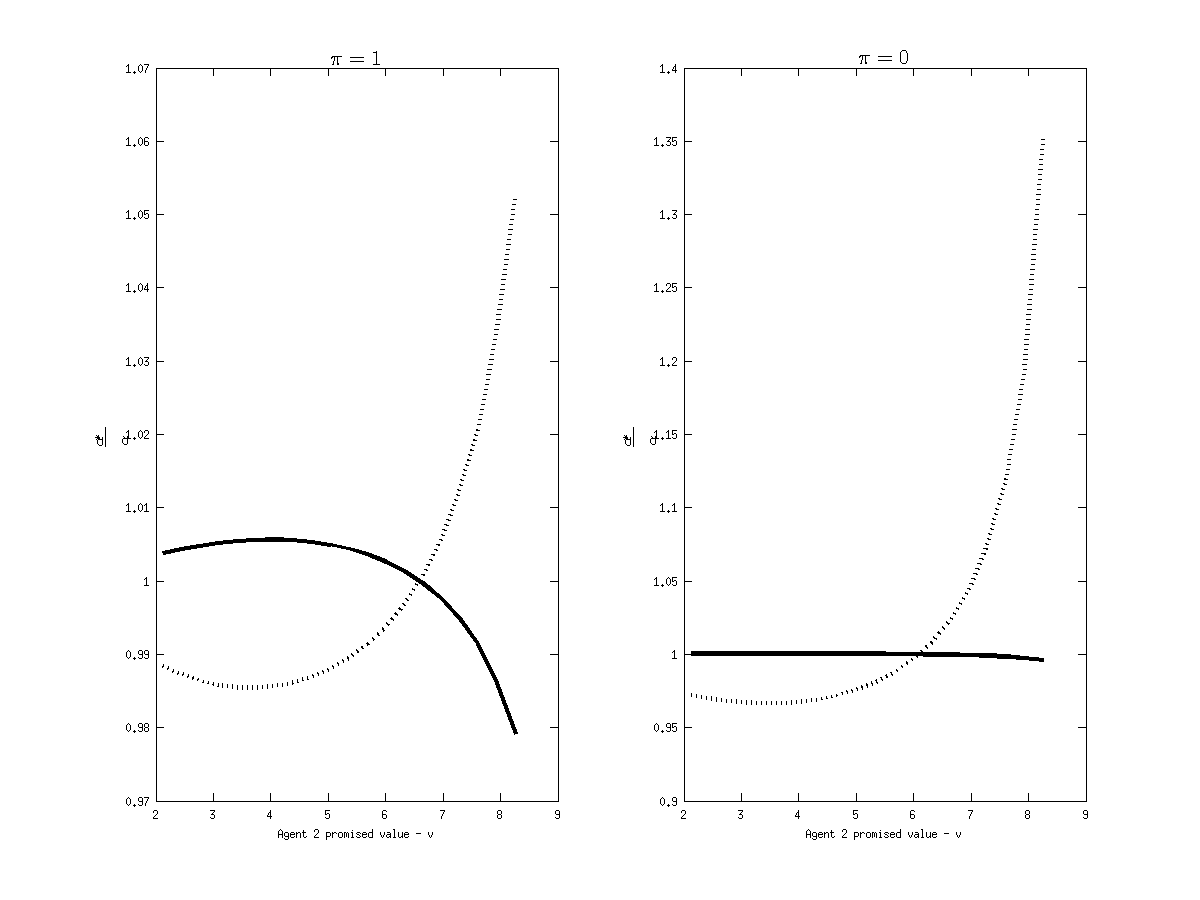
\includegraphics[scale=0.4]{Matlab/InfiniteHorizon/Learning/Plots/theta_1_finite/Transitory/AlphaStarNoLearning.png}

	\caption{\scriptsize{This figure plots the gross change in consumption shares as a function 
of the initial promised value to Agent 2 given $y(z)=y_l$. The solid (dotted) line refers to
 $y(z^*)=y_l (y_h)$. The left (right) panel is the IID Model with $\pi=1$ ($\pi=0)$}}
	\label{fig:AlphaStarNoLearning}
\end{figure} 
\hyperlink{ResultsComMarket}{\beamergotobutton{}}
\end{frame}
\begin{frame} [label=ConsSharesAmb2]
\frametitle{Consumption Shares - Ambiguity (II)}
\begin{figure}[htbp]
\centering
	  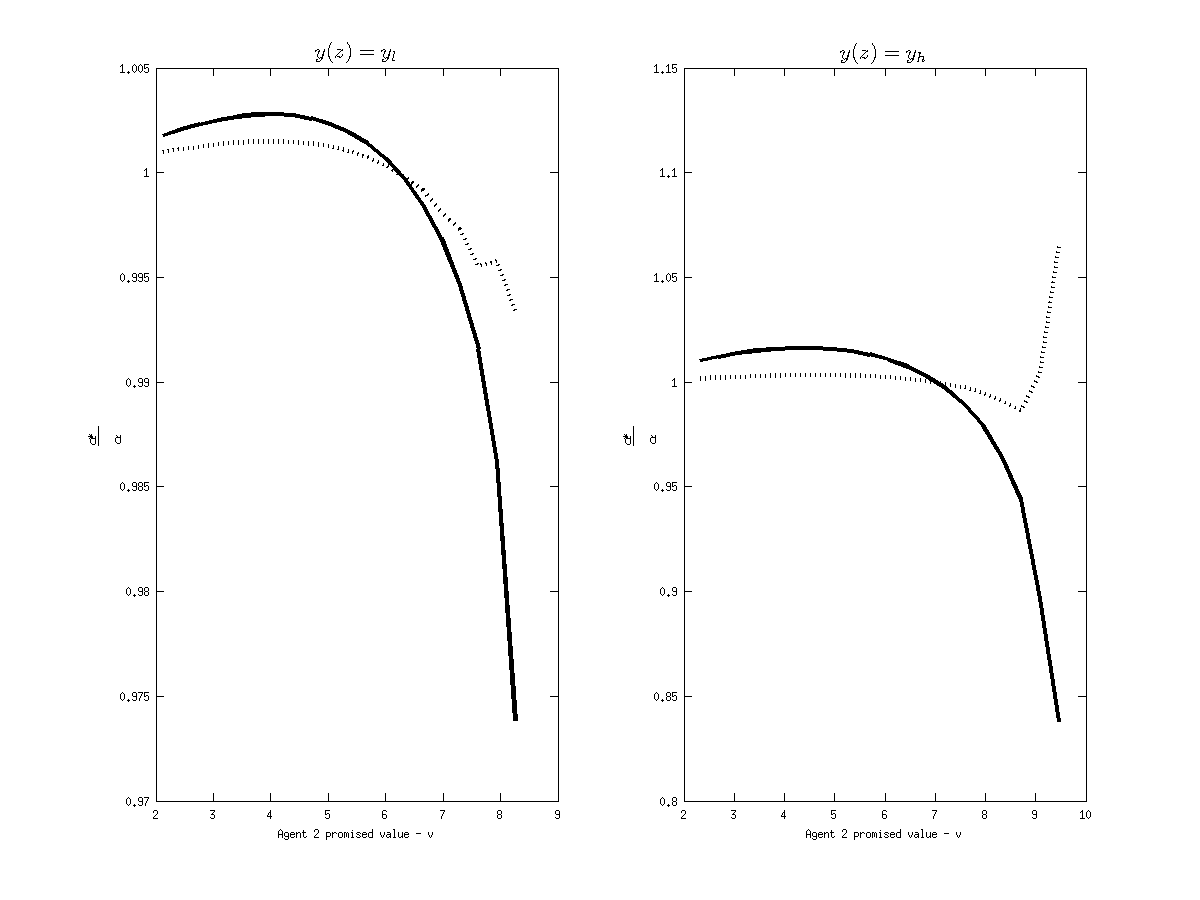
\includegraphics[scale=0.4]{Matlab/InfiniteHorizon/Learning/Plots/theta_1_infty/Transitory/AlphaStarLearning.png}

	\caption{\scriptsize{ This figure plots the gross change in consumption shares as a function 
of the initial promised value to Agent 2 - v keeping $y(z^*)=y(z^{**})$ and $\pi=0.5$. The solid (dotted) line refers to
 $s(z^*)=s_l (s_h)$. The left (right) panel is the $y(z)=y_l(y_h)$}}
	\label{fig:AlphaStarLearning}
\end{figure} 
\hyperlink{ResultsComMarket}{\beamergotobutton{}}
\end{frame}

\begin{frame}[label=RelEntropy]
\frametitle{Relative Entropy}
\small{\[\mathcal{E}_{P,Q} =  \mathbb{E} \frac{\tilde{p}^i(z^*|z,\pi)}{p(z^*|z,\pi)} \log\left[\frac{\tilde{p}^i(z^*|z,\pi)}{p(z^*|z,\pi)}\right]\]}
\begin{figure}[htbp]
\centering
	  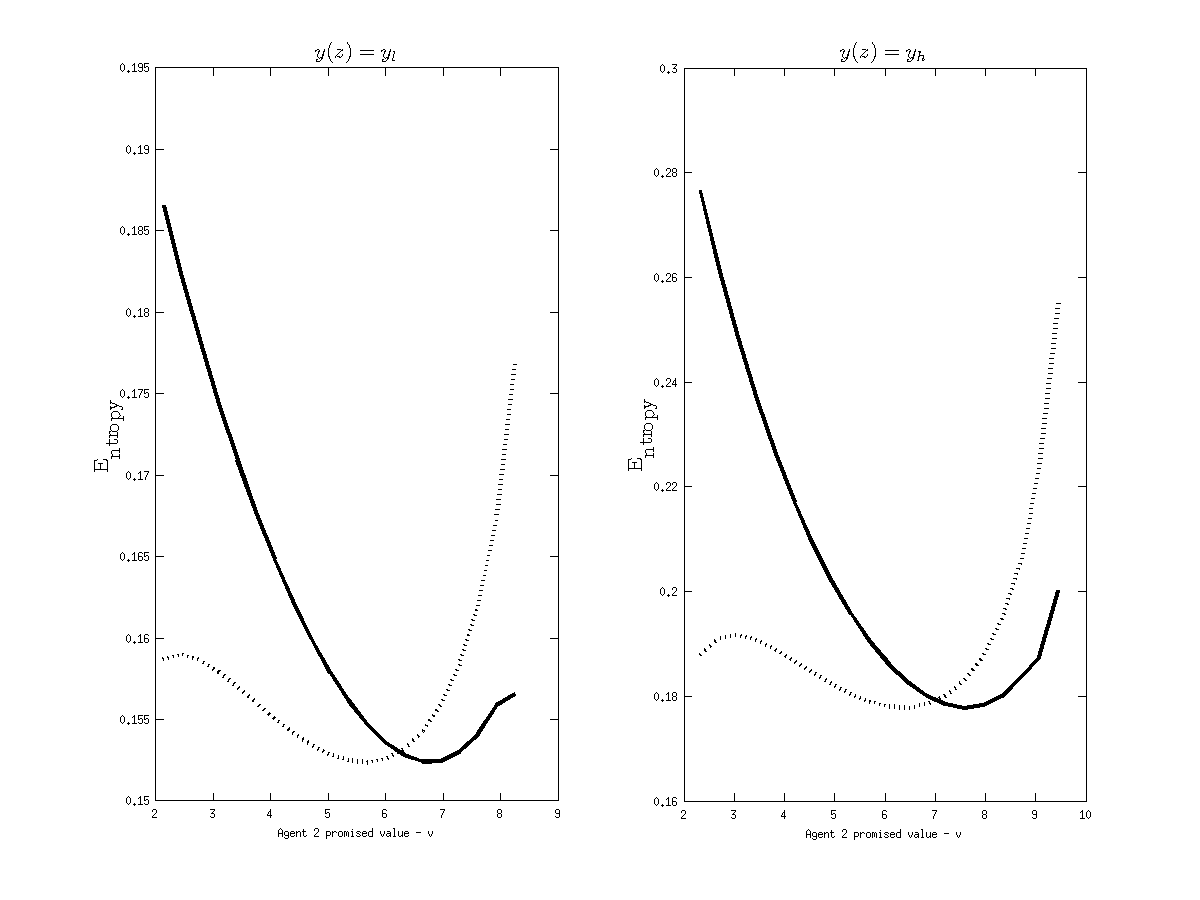
\includegraphics[scale=0.35]{Matlab/InfiniteHorizon/Learning/Plots/theta_1_finite/Transitory/EntropyMarginal.png}

	\caption{\scriptsize{This figure plots the relative entropy of the model averaged
 conditionals for both the agents. The solid (dotted) line refer to Agent 1 (Agent 2). The left (right) panel has $y(z)=y_l (y_h)$ and $\pi=0.5$ }}
 
	\label{fig:EntropyMarginal}
\end{figure} 
\hyperlink{ResultsComMarket}{\beamergotobutton{}}
\end{frame}

\begin{frame} [label=MPRNoLearning]
\frametitle{Market Price of Risk}
\begin{figure}[htbp]
\centering
	  \includegraphics[scale=0.4]{Matlab/InfiniteHorizon/Learning/Plots/theta_1_finite/Transitory/MarketPriceofRiskNoLearning.png}

	\caption{\scriptsize{This figure plots the MPR as a function of the initial promised
value to Agent 2- v. The  solid (dotted) line refers to $y(z)=y_l (y_h)$. The
left (right) panel has $\pi=1 (\pi=0)$}}
	\label{fig:MPRNoLearning}
\end{figure} 
\hyperlink{ResultsComMarket}{\beamergotobutton{}}
\end{frame}
\begin{frame}[label=MPRLearning]
\frametitle{Market Price of Risk - $\pi$} 
\begin{figure}[htbp]
\centering
	  \includegraphics[scale=0.4]{Matlab/InfiniteHorizon/Learning/Plots/theta_1_infty/Transitory/MPRLearningPi.png}

	\caption{ \scriptsize{This figure plots the conditional market price of risk as function of $\pi$ for $v\approx v^{max}$ . The solid (dotted) line is $y(z)=y_l (y_h)$. The left panel has $\theta_2<\infty,\theta_1=\infty $ and the right panel has both $\theta_1,\theta_2=\infty$}}
 
	\label{fig:MPRLearningPi}
\end{figure} 
\hyperlink{ResultsComMarket}{\beamergotobutton{}}


\end{frame}

\begin{frame}[label=LambdaNoLearning]
\frametitle{Changes in $\lambda$}
\begin{figure}[htbp]
\centering
	  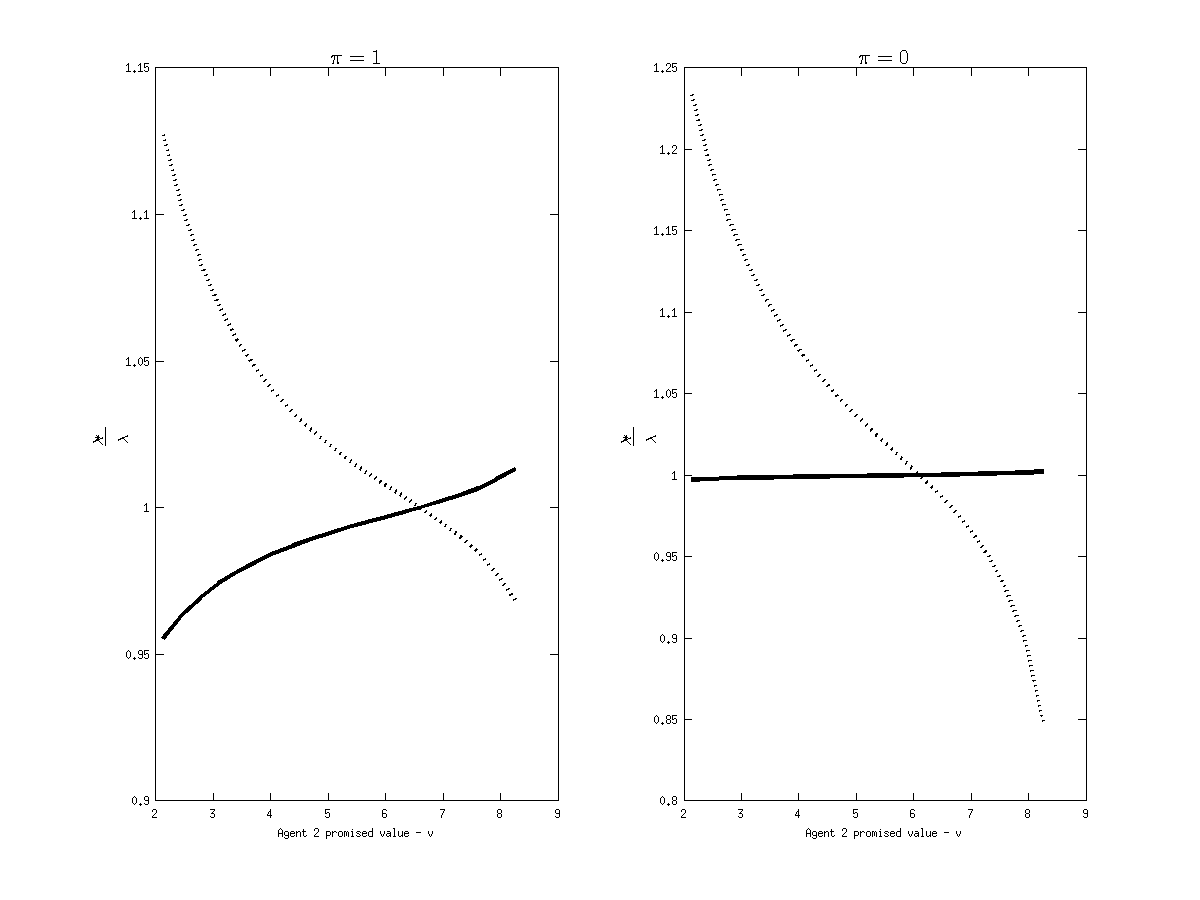
\includegraphics[scale=0.4]{Matlab/InfiniteHorizon/Learning/Plots/theta_1_finite/Transitory/LambdaStarLNoLearning.png}

	\caption{\scriptsize{This figure plots the gross change in implicit Pareto weights as a function 
of the initial promised value to Agent 2 given $y(z)=y_l$. The solid (dotted) line refers to
 $y(z^*)=y_l (y_h)$. The left (right) panel is the IID Model with $\pi=1$ ($\pi=0)$}}
	\label{fig:LambdaStarLStarNoLearning}
\end{figure} 
\hyperlink{ResultsComMarket}{\beamergotobutton{}}
\end{frame}

\end{document}	



